\documentclass[11pt,preprint]{aastex}
\usepackage[top=1in, bottom=1in, left=1in, right=1in]{geometry}
%\usepackage{natbib}
%\usepackage{natbibspacing}
\usepackage{enumitem}
\usepackage{url}
\usepackage{xcolor}
\usepackage{wrapfig}
\usepackage{float}
%\graphicspath{{figures/}}
\usepackage{amsmath, amssymb}
%\usepackage{subcaption}
\setlist[itemize]{noitemsep, topsep=0pt}
\setlist[enumerate]{noitemsep, topsep=0pt}
%\setlength{\bibspacing}{0pt}
\setlength{\parskip}{0pt}
\setlength{\parsep}{0pt}
\setlength{\headsep}{6pt}
\setlength{\topskip}{0pt}
\setlength{\topmargin}{0pt}
\setlength{\topsep}{6pt}
\setlength{\partopsep}{0pt}
\setlength{\footnotesep}{8pt}
\usepackage{titlesec}

\titlespacing*{\section}{11pt}{11pt}{3pt}
\titlespacing*{\subsection}{22pt}{6pt}{3pt}
\titlespacing*{\subsubsection}{33pt}{3pt}{3pt}


\begin{document}
\def\simlt{\lower.5ex\hbox{$\; \buildrel < \over \sim \;$}}
\def\simgt{\lower.5ex\hbox{$\; \buildrel > \over \sim \;$}}
\def\wLO{\omega_0}

\title{LAB 1: Digital Sampling, Fourier Filtering, and Heterodyne Mixers in Radio Astronomy}

\tableofcontents

\section{Introduction}

\noindent
In this lab, we delve into digital samplers, discrete Fourier Transforms, and
mixers---key tools in radio astronomy and everyday technologies like cell
phones, radios, and televisions. Did you know WiFi was developed by a radio
astronomer?

This series of experiments will introduce you to the practical aspects of radio
astronomy. You'll configure lab equipment, collect and analyze data, and
present your findings. The skills and pipeline you develop here are crucial for
Lab 2, where you'll observe hydrogen's 21-cm line emission in the Milky Way.
Save yourself \textbf{technical debt} by investing in your understanding and your code base.

Success in this lab hinges on establishing good research practices. Your grade depends on the report due three weeks from now, crafted from the exercises and data you'll gather. While completing every task isn't mandatory, your report should thoroughly address the goals outlined in \S\ref{goals}.

To enhance your lab experience and report:

\begin{itemize}
    \item Maintain a \textbf{lab notebook}. Detailed notes on your experimental setup are vital for interpreting data and troubleshooting. We can't help you if you can't remember your experimental configuration!
    \item \textbf{Revision control} your data, code, and plots. This safeguards against data loss and facilitates reproducibility.
    \item Begin your report early. Planning for the data and plots you need helps optimize lab time and reduces last-minute stress. Write incrementally to avoid facing a blank page.
    \item Use lectures, AstroBaki, the internet, and these instructions as resources. When it comes to research and making things work, you have to move beyond the textbook to find trustworthy resources. Exploration and note-taking are key.
    \item Aim for the style of scientific publications. Your report should guide the reader to understand and trust your results, focusing on the synthesis of findings rather than a detailed chronicle of your process. Ensure all words and plots in your report are original. Cite external sources.
\end{itemize}


\section{Goals} \label{goals}

\noindent
The objectives of this lab, which your report should demonstrate, include:

\begin{itemize}
    \item Sampling electronic signals and converting them to digital format. Show aliasing effects and quantitatively link them to the Nyquist criterion.
    \item Effective use of Discrete Fourier Transforms (DFTs) for analyzing frequency power spectra from voltage data. Ensure correct calculation and labeling of frequency and power axes, understanding frequency ranges and resolutions in relation to sample duration and cadence.
    \item Understanding negative frequencies and how complex inputs in Fourier Transforms to distinguish positive/negative frequencies.
    \item Identifying and analyzing noise in electronic measurements, including its behavior under Fourier Transform.
    \item Applying the convolution/correlation theorem to explain spectral leakage in power spectra and to explore the relationship between power spectra and autocorrelation functions.
    \item Using heterodyne mixing for frequency conversion, assessing the differences between real and ideal mixers. Experiment with double- and single-sideband mixers, demonstrating their theoretical and practical variations.
\end{itemize}

\noindent
Your report will be evaluated based on your presentation of theoretical background, experimental setup, data analysis, and the quantitative interpretation of results in these areas.

Additionally, the report will reflect your proficiency in the following technical skills, which do not need explicit discussion:

\begin{itemize}
    \item Configuring lab equipment and operating Linux on Raspberry Pi.
    \item Using Python for experimental control, data acquisition, analysis, signal processing, and plotting.
    \item Writing a technical report in \LaTeX, including abstracts, figures, tables, and citations.
\end{itemize}


\section{Schedule}

\noindent
This is an ambitious lab with a steep learning curve.
Do not to get behind or backload your work schedule.
Students always underestimate how long it takes to write a report.

\begin{enumerate}
    \item {\it Week 1:} Complete \S \ref{nyquist} and review \S \ref{pwrspectrum}. Be ready to demonstrate your work, software, and results in class.
    \item {\it Week 2:} Finish \S \ref{mixersect} and go through \S \ref{hetereo}. Prepare to present your findings and progress to the class.
    \item {\it Week 3:} Consult \S \ref{report} for report-writing guidance. Focus on crafting a formal report that effectively addresses the objectives in \S\ref{goals} and adheres to the norms of scientific writing. Your report will be graded on its quality and adherence to scientific publication standards.
\end{enumerate}



\section{Software Engineering}

\noindent
The programming complexity of these labs increases throughout the semester.
You will need to develop good practices in organizing, documenting, testing, and
stabilizing your code. Software engineering is a vital (and highly marketable) skill, and we begin with
these principles:

\begin{itemize}
    \item {\it Package your code}: Move beyond Jupyter notebooks by building infrastructure code (functions and classes) into {\bf modules} and {\bf packages}. This separation enhances organization, testability, and reusability. See \url{https://docs.python.org/3/tutorial/modules.html} for guidance.
    \item {\it Code (at least) twice}: First, code to understand your program's functionality. Then, recode for better organization. Thoughtful interface design is crucial to good coding, as it limits complex dependencies, enhances usability, and speeds debugging.
    \item {\it Test your code}: How do you know your code works? What defines success?  In software as in science, you can only {\it expect} what you {\it inspect}, which is to say that you can only trust something work to the extent that you have tested that it does so.
Modular testing, or {\bf unit testing}, is key in large projects. Python's {\tt unittest} module presents a good starting point.
    \item {\it Control your revisions}: Use revision control tools like {\tt git} to track code changes. A GitHub account can facilitate code backup, synchronization across devices, and collaboration. Embrace the learning curve---it's worth it.
\end{itemize}

\noindent
In advanced software engineering, online repositories host branches of a project, with continuous integration systems running unit tests. While we won't use these advanced methods in this class, understanding them is beneficial.

Separate data acquisition (lab and telescope control) from data analysis. Use command line scripts for acquisition and Jupyter notebooks for analysis. For shared code, create modules importable in both environments.


\section{Digitally Sampling a Sine Wave (Lab Activity, Week 1)}
\label{nyquist}

\subsection{Handouts and Software}

\noindent
Your first week's tasks involve exploring digital sampling and spectral
analysis while using Linux and Python programming. Refer to
Astrobaki\footnote{\url{https://casper.astro.berkeley.edu/astrobaki/index.php/Undergraduate_Radio_Lab}}
to review key course topics ({\it Nyquist Sampling} and {\it The Fourier
Transform}), and for primers on Linux/Unix, Python Installation and Basic
Programming, Unix Text Editors (ViM/Emacs), and Revision Control.

\subsubsection{The {\tt ugradio} Python Package}

\noindent
The {\tt ugradio} package contains supporting code for the labs. It is pre-installed on the provided SD card for your Raspberry Pi. To verify, open {\tt ipython} or a {\tt jupyter notebook} and try {\tt import ugradio}. Installation on other computers is possible via GitHub, linked on the course website.
Focus on {\tt ugradio.sdr} and {\tt ugradio.dft} modules.

\begin{itemize}
    \item {\tt ugradio.sdr} --- For interfacing with the Software-Defined Radio (SDR) receiver on your Raspberry Pi.
    \item {\tt ugradio.dft} --- Offers functionality for arbitrary Discrete Fourier Transforms, in contrast to {\tt numpy.fft}, which is limited to specific types but operates (much) faster.
\end{itemize}

\noindent
Explore these modules on GitHub, in the {\tt ugradio/ugradio\_code/src} directory on your Raspberry Pi, or within Jupyter/IPython using {\tt ??} after a module, function, or class name.




\subsection{Digital Sampling and the Nyquist Criterion}

\noindent
Explore the Nyquist criterion for discrete sampling by using a Software-Defined Radio (SDR) module with a Raspberry Pi, and through Python simulations. Vary the signal frequency ($\nu_0$) and sampling frequency ($\nu_s$), comparing results with theoretical expectations. Your report should include a focused analysis of aliasing that integrates theory, data analysis, and simulations.
Try to pose and quantitatively answering a specific question.
``{\it What is aliasing}" is too broad. ``{\it How many Nyquist zones
can I demonstrate using my RPi SDR module}" is a tighter framing with
a quantifiable answer that you can provide evidence to support. Even better
would be ``{\it using (purposeful) aliasing, can I characterize
the bandpass filter inside my SDR module?}"

\subsubsection{Sampling with an SDR and a Raspberry Pi}

Get a prepared SD card or follow the setup instructions on AstroBaki for {\it Setting Up Your Raspberry Pi}. Once set up, connect an SDR (like Nooelec NESDR SMART) to the USB (blue = 3.0 = faster) port. Regularly update the {\tt ugradio} package to ensure its latest version:
\begin{enumerate}
    \item {\tt cd ~/ugradio/ugradio\_code}
    \item {\tt git pull}
    \item {\tt pip install .}
\end{enumerate}

For an optional demonstration that uses the capabilities of the R820T2 tuner chip and the RTL2832U quadrature digital sampler chip, connect an antenna to the SDR input and use {\tt gqrx} to listen to FM radio broadcasts. 
Under {\tt I/O Devices} set {\tt Device String} to 

\noindent
{\tt default\_input=True,default\_output=True,device\_id=0,driver=audio}, 

\noindent
then press {\tt Play}. 
Fiddle with the settings (e.g., use Hardware Automatic Gain Control, WFM Stereo demodulation), and
you should be able to listen to Frequency Modulated (FM) 
radio, which in the US spans 87.8--108 MHz, by setting an appropriate center frequency.

Listening to FM broadcasts is fun, but we need to know what happens between the antenna and the speaker.
For starters, we will bypass most everything and just use the analog-to-digital converter (ADC) inside the RTL2832U.
This mode is called {\bf direct sampling} in the {\tt ugradio.sdr} module.
Use a signal generator to produce a $<500$ kHz sine wave with a $<3$ mV peak-to-peak voltage (using an attenuator if necessary).
Verify the signal with an oscilloscope (mantra: mistrust everything!) and document your settings before plugging it into your SDR.

Write Python code to create an {\tt ugradio.sdr.SDR} object and capture data with varying sample rates ($\nu_s = 1.0$--3.2 MHz).
Plot your captured data (which is a {\it multidimensional} {\tt numpy} array) to make sure it looks sinusoidal.
{\it Your first data capture can sometimes contain a stale (old) buffer, so inspect your data carefully.}
Observe how the sine wave's amplitude changes with frequency due to internal filters in the RTL2832U, which are designed to suppress aliasing.
You can override these filter settings
\footnote{If you are curious, 
I expanded the {\tt librtsdr} driver and {\tt pyrtlsdr} Python wrapper
to support setting the coefficients of a Finite Impulse Response
(FIR) filter. FIR filters implement convolutional filters, which we will
learn about next week.}
to illustrate aliasing more clearly using
{\tt fir\_coeffs=np.array([0, 0, 0, 0, 0, 0, 0, 0, 0, 0, 0, 0, 0, 0, 0, 2047])}.

Investigate different Nyquist zones and the RTL2832U's filter response by experimenting with various $\nu$ values. Document your methods, equipment details, and signal settings. Compare aliased amplitudes with default and enhanced aliasing settings.

Write plain text scripts to collect and save data arrays (and metadata) using {\tt numpy.savez}. Load files into Jupyter notebooks with {\tt numpy.load} and use {\tt matplotlib} to interactively plot and inspect the sampled waveforms. 
Explore the Fourier spectrum of your signals with either {\tt numpy.fft} or {\tt ugradio.dft} and compute the power spectrum (see \S\ref{dft} and \S\ref{pwrspect}).
For Fourier plots, pay particular attention to data order (e.g. {\tt numpy.fft.fftshift}) and units, both in frequency and amplitude.

When you have plots you like in your Jupyter notebook, graduate them to revision controlled, plain-text scripts that you can use to reliably reproduce them from raw data for your report.
Make sure to label all axes (with appropriate units to avoid tiny or huge numbers)
give it a title, and restrict the range to clearly illustrate
the signal shape and frequency.
Your report will need include an appropriate caption that
stands alone as a description of the plot and what it demonstrates.

Try producing a plot that synthesizes several data runs to illustrate aliasing and Nyquist's criterion.
You will produce and plot more data than you should put in your report.
Make sure the ones in your report are focused on quantitatively illustrating a point.
One good plot is worth more than many vague ones.


\subsection{Voltage Spectra and Power Spectra}

\noindent
Understanding the difference between power and voltage spectra is vital.
Power spectra summarize the frequency content of our signal, while voltage spectra provide additional phase information with real and imaginary components.
Why might power spectra be preferred over voltage spectra, or vice versa?

Consider the complex nature of voltage spectra. What do the real and imaginary numbers signify? What are negative frequencies, and how are they realized in your data? These concepts can be explored in your lab report.

From your previous data, plot both real ({\tt spec.real}) and imaginary ({\tt spec.imag}) components of the voltage spectrum. Observe any symmetry between negative and positive frequencies. Repeat this with independent data to verify consistency. Analyze why the real and imaginary parts vary in amplitude and sign.

Using {\tt dft.idft} or {\tt numpy.fft.ifft}, perform an inverse Fourier Transform of a {\it power} spectrum .
Ensure correct frequency inference for each bin in your power spectrum array. Also, compute the autocorrelation function (ACF) from the voltage time series using {\tt numpy.correlate} and {\tt scipy.signal.correlate}. 

According to the correlation theorem, the Fourier transform of the power spectrum should match the ACF. Compare them and explain any discrepancies.


\subsection{Leakage Power} \label{subleakage}

\noindent
When using {\tt dft}, the default setting calculates a power spectrum at $N$ frequencies for a signal with $N$ time samples, where each frequency is separated by $\Delta\nu = \nu_s/N$. 
For Fast Fourier Transform (FFT) operations like {\tt numpy.fft}, this time/frequency sample correspondence is hard-coded.

For this exercise, calculate the power spectrum of some captured waveforms with $N_{\rm freq}\gg N$, diverging from the guidelines in \S \ref{dft}.
Use {\tt dft} with frequency increments $\Delta \nu \ll \nu_s/N$. Employ a logarithmic vertical axis to identify if there is non-zero power at frequencies other than $\nu_0$. The presence of power at $\nu\ne\nu_0$ indicates \textbf{spectral leakage}, a common phenomenon in Fourier-based power spectra calculations. 

Take a look at the Convolution Theorem. Can you explain mathematically why you might find power at $\nu\ne\nu_0$ using a Discrete Fourier Transform?


\subsection{Frequency Resolution} \label{freqres}

\noindent
Determine how closely spaced two spectral lines (sine waves) can be while still being distinguishable.

Combine the outputs of two function generators using a power splitter (used in reverse as a combiner). Select two frequencies very close together and plot their power spectrum, ensuring the frequency points are more densely spaced than the standard $\Delta \nu = \nu_s/N$.

Experiment, for a fixed number of time samples, to find the minimum frequency separation where the two signals remain resolvable---this gap is the \textbf{frequency resolution}. Examine how this resolution is affected by the number of samples in the Discrete Fourier Transform (DFT). How does it relate to the time interval spanned by those samples?

Conclude by providing a mathematical explanation for your experimental findings regarding frequency resolution.
Again, can you interpret this result using the Convolution Theorem?


\subsection{Power Spectra in other Nyquist Windows}

\noindent
This exercise extends the exploration of power spectra beyond the standard frequency range of $\pm \nu_s/2$. 

Use a Nyquist-sampled time series to calculate power spectra over an expanded frequency range of $\pm W \nu_s/2$, where $W$ is at least 4, focusing on the original frequency interval.
Each value of $W$ represents a different \textbf{ Nyquist window}.
Compare the power spectra obtained across these various Nyquist windows.
For $W > 1$, the power spectra include frequencies that seemingly violate the Nyquist criterion, yet they produce interpretable results. In Lab 4, for instance, our digital spectrometer will operate in the 12$^{\rm th}$ Nyquist window.

This investigation illustrates a more nuanced interpretation of the Nyquist criterion: it is the signal's {\it bandwidth}, inclusive of negative frequencies, that must not exceed $\nu_s$.


\subsection{Fourier Transforms of Noise}

\noindent
Noise, in scientific data, refers to random fluctuations with a known statistical distribution, typically Gaussian.
This is distinct from systematic errors, bias, ambiguity, or posterior likelihood.
Unlike how we use the term colloquially, noise has a specific meaning in science, so be careful with it.

Many astronomical signals are essentially noise. Consider blackbodies, which emit electromagnetic waves with intensities described by the Planck function:
\begin{equation}
B_\nu = \frac{2h\nu^3}{c^2}\frac{1}{e^{h\nu/kT}-1}.
\end{equation}
In radio astronomy's Rayleigh-Jeans limit ($h\nu/kT \ll 1$), this simplifies to:
\begin{equation}
B_\nu\approx\frac{2kT}{\lambda^2},
\end{equation}
highlighting the linear dependence of noise power on temperature $T$.

Radio astronomers often express noise power in terms of temperature, using brightness temperature $T_B$ such that $I\equiv2kT_B/\lambda^2$. This applies even if the radiation source, like galactic synchrotron emission, is not thermal.

All power sources in measurements can thus be related to a temperature, including receiver noise.
Receiver noise, for example, is added to our incoming astronomical signal 
by the thermal motion of electrons in our amplifiers and resistors 
(otherwise known as {\bf Johnson} noise).  This noise (which,
by the Central Limit Theorem, is almost always Gaussian) has a variance that
is characterized by receiver temperature, $T_{rx}$, and adds onto the brightness temperature, $T_B$, 
that characterizes the variance of signal coming through the antenna feed of the telescope.

Our lab has various noise sources that can be used to explore the properties of digitally sampled noise.


\subsubsection{Use the Laboratory Noise Generator}

\noindent
The lab's noise generator produces broadband, random voltages using a diode. To prevent aliasing, connect a band-pass filter before performing direct sampling with your SDR module. Determine an appropriate sample rate to avoid aliasing.

\begin{itemize}
    \item Connect the noise generator to a filter and capture tens of thousands of samples with the SDR's ADC. Analyze the mean and variance of these voltage samples.
    \item Create a histogram of the sampled voltages using {\tt numpy.histogram}. It should approximate a Gaussian distribution with a width equal to the rms voltage. Overplot a theoretical Gaussian for comparison. Explain any differences.
    \item Collect multiple data blocks (tens to hundreds), each containing thousands of samples. Compute the power spectrum for each block and the average power spectrum across all blocks.
    \item Compare the power spectrum of a single block to the average over $N$ blocks where $N=(2, 4, 8, 16)$. Investigate how time averaging influences the signal-to-noise ratio (SNR). Determine if SNR scales with $N^x$ and how this compares to predictions from the Central Limit Theorem.
    \item Calculate the Autocorrelation Function (ACF) for a 16000 sample block, both manually and using {\tt numpy/scipy}. Focus on delays of $\le 2000$ samples. How does the power spectrum computed from the ACF compare with that obtained via Fourier transform? Assess their similarity, and compare the full-width half-max (FWHM) of the ACF ($\Delta \tau_{FWHM}$) with the FWHM of the power spectrum ($\Delta F_{FWHM}$). Are they related?
\end{itemize}


%=============================================================
\section{Fourier Transforms, Analytic and Discrete (At Home, Week 1)} 
\label{pwrspectrum}
 
\subsection{The Analytic Fourier Transform}

\noindent
A Fourier transform maps a function between two complementary coordinates which
for now are usually time, $t$, and spectral frequency, $\nu$.
The input to a forward Fourier transform is a signal versus time, 
$E(t)$; the output is a signal versus frequency, $\tilde E(\nu)$,
which is computed as
% 
\begin{equation}
\tilde E(\nu) = \int_{-T/2}^{T/2} E(t) e^{-2 \pi i \nu t} dt \ .
\label{eq:dft}
\end{equation}
% 
\noindent The input signal $E(t)$ is multiplied by a complex
exponential and integrated, so the $\tilde E(\nu)$ is a complex-valued function. Of particular
importance is that the Fourier Transform is {\bf invertible}: 
you can get back to the time domain using the inverse transform
%
\begin{equation}
E(t) = {1 \over B} \int_{-B/2}^{B/2} \tilde E(\nu) e^{2 \pi i \nu t} d\nu \ .
\end{equation}
% 
This works because (complex) sine waves form a {\bf basis} over the space of functions.
Any function can be expressed exactly and uniquely by its Fourier coefficients
\footnote{You may wonder how
the integration limits $B$ and $T$ are defined above. In the proper
analytic formulation, they are both infinity. We emphasize their
boundedness here because, in practice, 
neither can be infinity, and this unavoidably introduces spectral leakage. Also note that,
according to the Fourier conventions we've written here, our forward FT does not divide
by the integration interval, but the inverse FT does.  These conventions match 
the {\tt numpy.fft}/{\tt ifft} conventions.}

For those of you looking to apply that linear algebra class you took,
the Fourier transform (FT) is a linear matrix operator akin to a rotation. 
As such, it has nice properties like:
\begin{enumerate}
\item linearity: the FT of a sum is the sum of the FTs, 
\item invertibility: there is no information loss in the FT; it can be undone, and 
\item unitarity: the FT is power-preserving.
\end{enumerate}


\subsection{The Discrete Fourier Transform (DFT)} \label{dft}

\noindent
The difference between an analytic Fourier transform and a discrete Fourier transform is
that signals sampled at discrete intervals are no longer continuous. 
Integrals become sums, and the Nyquist criterion applies.

You have multiple discrete Fourier transform implementations at your disposal.  Eventually, we would like you
to use \verb$numpy.fft$, which is fast (it can handle millions of points), but does not allow you to choose
which frequencies are in your output. It also has the (sensible but confusing) feature that, in the output
spectrum puts the zero frequency in the 0th array index, counts upward through the positive frequencies, then
switches in the middle to the most negative frequency and continues counting in the positive direction
toward zero.  The inverse Fourier transform \verb$numpy.fft.ifft$ requires the input spectrum to be in this
order to work properly.

However sensible, this arrangement of frequencies is not ideal for plotting. The function \verb$fftshift$
will swap the order to a plot-friendly negative-to-positive order. However, once you apply this shift to
your array, \verb$ifft$ no longer works as you expect.  For this reason, {\it I strongly suggest only using 
\verb$fftshift$ in plotting calls.}
See our ``DFT's with DFT's'' handout for details.

You should also take a look at \verb$fftfreq$, which calculates the frequencies of the \verb$numpy.fft$ output.

For this class, we also provide the \verb$ugradio.dft$ module.  It is slow, but it allows you to manually specify
which output frequencies are desired, and it accepts and returns coordinate arrays (time and frequency, respectively)
to facilitate clarity and transparency. You can use this module in the first week and for applications where
you need to oversample the output frequencies. Otherwise, migrate to \verb$numpy.fft$.

To use \verb$ugradio.dft$, here are some recommendations:
\begin{itemize}

\item The set of sample times, $N$. Modern FFT libraries allow for arbitrary $N$, but performance improves
if $N$ has small prime factors. 
It is also advantageous to use even values of $N$, so that the zero frequency falls in the center of a bin.
Powers of two are common. 
Our \verb$dft$ module is slow, though, and this won't help. 

\item Define the time range so that $t=0$ falls at the center of the range.
  For $N$ even, there is no center time, so make the times
  run from $-\frac{N}{2}/ \nu_s$ to $(\frac{N}{2} -1)/ \nu_s$.

\item 
  In specifying the frequencies for which you want the output $\tilde E(\nu)$, I 
  suggest that you first calculate the output for $N$
  frequencies running from $-\frac{\nu_s}{2}$ to $+\frac{\nu_s}{2}\left(1 - \frac{2}{N} \right)$. 
This makes the frequency
  increment equal to $\Delta \nu = \nu_s/N$ over a total range of
  just under $\nu_s$.

\end{itemize}

To find out how to use the DFT, you can type {\tt ugradio.dft.<tab>} to see an
auto-complete of what is available in the module.  You can also type {\tt ugradio.dft??} to see
the code, and of course, you can type {\tt ugradio.dft.dft?} to see the documentation for
the DFT function inside the {\tt dft} module.

\subsection{(Optional) Fourier Filtering and a Secret Message}

As an optional (fun) side investigation you can do on your own at
home 
with Fourier filtering, we have provided an audio message encoded as a {\tt numpy} array in the 
{\tt secret\_message.npz} file. This file holds the waveform ({\tt 'data'}) and the sample
frequency ({\tt 'fs'}). If you install the python module {\tt sounddevice} on {\bf your home computer}:
\begin{verbatim}
$ pip install sounddevice
\end{verbatim}
you can record (from {\it your home} microphone):
\begin{verbatim}
>>> import sounddevice as sd
>>> import scipy.io.wavfile
>>> seconds = 3 # s, recording duration
>>> fs = 44100 # Hz, sample rate
>>> recording = sd.rec(int(seconds * fs), samplerate=fs, channels=1) # record from microphone
>>> sd.wait() # wait for recording to finish
>>> scipy.io.wavfile.write('output.wav', fs, recording)
\end{verbatim}
and play data (from {\tt numpy} arrays!):
\begin{verbatim}
>>> fs, data = scipy.io.wavfile.read('output.wav') # read wav file to numpy array
>>> sd.play(data, fs) # play to speaker
>>> sd.wait() # wait until finished playing
\end{verbatim}
In this case, however, we've stored the data in a {\tt npz} file, not a {\tt wav} file, so you
don't need to use $\tt scipy$ to read it.

The data we have provided contains a secret audio message, but with high-frequency noise
overlaying it that makes it hard to hear. See if you can use a power spectrum to characterize
what frequencies cointain the high-frequency noise, then filter the voltage spectrum, transform
back to a time-domain function (because Fourier transforms are invertible!) and play the secret
message.


\subsection{Power Spectra and Discrete Fourier Transforms} 
\label{pwrspect}

\noindent
We are often interested in the output {\bf power spectrum}, 
$P_\nu$.  Power is proportional to voltage squared.  For complex quantities, the squaring
operation means we want the sum of the squares of the real and imaginary
parts.  We obtain this by multiplying the voltage by its complex
conjugate (denoted by `$^*$'),
%
\begin{equation}
P_\nu = \tilde E(\nu) \tilde E^*(\nu) \ .
\end{equation}
% 
\noindent In Python, there are two ways to get this product.  One is to use
the \verb$conj$ function, i.e.\ {\tt P = E * E.conj()}.  Should the
imaginary part of \verb$P$ be zero? (answer: yes! Why is this?) Is it?
(answer: not always! Why not?) To get rid of this annoying and extraneous
imaginary part, try casting your array as a float.
 
The other (more convenient and suggested) way is to square the length of
the complex vector, i.e.\ \verb$P = numpy.abs(E)**2$. The result is
automatically real.


\subsection{The Power Spectrum and the Autocorrelation Function
  (ACF)} \label{acf}

\noindent
Facility with the {\bf convolution theorem} and its cousin,
the {\bf correlation theorem}, 
is a requirement for radio astronomy. 

The convolution of two functions $E$ and $F$ (here arbitrarily taken
to be functions of time) is
%
\begin{equation}
[E * F](\tau) = \int_{-T/2}^{+T/2} E(t) F(\tau - t) \ dt,
\end{equation}
%
and the correlation of the two functions is
%
\begin{equation}
[E\star F](\tau) = \int_{-T/2}^{+T/2} E(t) F(\tau + t) \ dt.
%\int_{-\infty}^{+\infty} E(t) F(\tau + t) \ dt
\end{equation}
%
\noindent Conceptually, these two functions describe sliding $F$ over
$E$ by changing the delay parameter, $\tau$, which describes a
time shift between the two functions.
The only difference between convolution and correlation is the sign of $t$ in the argument of
$F$.

Using our definition of the Fourier transform from
Equation \ref{eq:dft}, the convolution theorem states:
%
\begin{equation}
\widetilde{[E*F]}(\nu)\equiv\int_{-T/2}^{T/2} [E*F](\tau)~e^{2\pi i \tau\nu} d\tau =
    \tilde E(\nu) \cdot \tilde F(\nu)
\end{equation}
%
and the correlation theorem:
\begin{equation}
\widetilde{[E\star F]}(\nu)\equiv\int_{-T/2}^{T/2} [E\star F](\tau)~e^{2\pi i \tau\nu} d\tau =
    \tilde E(\nu) \cdot \tilde F^*(\nu)
\label{eq:acfpwr}
\end{equation}
%
In words, the theorem states that the Fourier transform of
  the convolution/correlation of two functions is equal to the product of their
  Fourier transforms (with one complex-conjugated for correlation).
If $F(t)$ is
symmetric, then the imaginary part of its Fourier transform is zero,
which means $\tilde F^*(\nu) = \tilde F^(\nu)$, and two theorems become
identical.

An important application of this theorem is the case when
$E(t)=F(t)$, in which the correlation function becomes the {\bf
  Autocorrelation function} $ACF(\tau)$, and equation \ref{eq:acfpwr}
states that the power spectrum is equal to the Fourier
  transform of the ACF.

Because of end/wrap-around effects, these theorems apply
strictly only in the limit $T \rightarrow \infty$.
When calculating a digital version of the correlation function, you have
to worry about end effects. Suppose you are calculating an ACF for $N$
samples with delays $\Delta N$ ranging up to $N/2$. Then the number of
terms in the sum is always smaller than $N$ because the delays spill
over the edge of the available samples. 

%So when you calculate the ACF you need to properly normalize:

%%XXX I don't think this equation clarifies matters
%\begin{equation}
%ACF(\Delta N) = { \Sigma_{k=0}^{ N-\Delta N-1} x_k x_{k+\Delta N} \over
%                  \Sigma_{k=0}^{ N-\Delta N-1} x_k^2}
%\end{equation}



\section{Mixers (Lab Activity, Week 2)} \label{mixersect}

\subsection{The Double-SideBand (DSB) Mixer} \label{sectdsb}

\noindent
In this section, you will build a double sideband (DSB) mixer (Figure \ref{dsb}).
A mixer is an electronic device that multiplies the two input signals. It is simple: the
radio frequency (RF) signal goes into one mixer port, the local oscillator (LO) goes into the second
mixer port, and the intermediate frequency (IF) product is output through the third port.

\begin{figure}[h!]
\begin{center}
  \includegraphics[height=2in]{dsbmixer.png}
\end{center}
\caption{\footnotesize A DSB mixer. In the text, we sometimes refer to
  the RF input as the `signal'. \label{dsb}}
\end{figure}

In our lab, we have Mini-Circuits ZAD-1 and ZFM-15 mixers. 
They have three BNC connectors
labeled R, L, and X or I, corresponding to
the RF, LO, and IF, respectively.
Both the ZAD-1 and the ZFM-15 are
balanced mixers, so the R and L ports are identical but
{\it will not couple to DC or very low frequencies}.  To find out
the frequency ranges these mixers support on each input, 
look up the datasheet online. 

%In contrast,
%the ``I'' port is coupled differently and will handle voltages all the
%way down to, and including, DC.  The mixing process functions no matter
%which two ports are used as inputs.  For example, if you are using a
%mixer to modulate a high frequency (say, a few MHz) with a low frequency
%(say, a few kHz), you should use the ``I'' port for the low frequency
%and either of the other two for the high frequency; take the output from
%the third port.  

Use a mixer to build a DSB.
Assign a signal generator to
be your LO with frequency $\nu_{LO}$ and
another to be your RF signal with frequency $\nu_{RF} = \nu_{LO} \pm
\Delta \nu$.  Here, you choose the frequency difference $\Delta \nu$ and
you set the two signal generators 
for each of two cases:
$\nu_{RF} = \nu_{LO} + \Delta \nu$ and $\nu_{RF} = \nu_{LO} - \
\nu$.  Make $\Delta \nu$ small ($\sim5$\%) compared to $\nu_{LO}$.
For the input power level, a good choice is 0
dBm\footnote{``dBm'' is the power relative to 1 milliwatt, expressed in decibels (dB).}
for both synthesizers. The output consists of both the
sum and difference frequencies, so choose the ports appropriately.

Digitally sample the mixer output and identify the
sum and difference frequencies.
Consider
the Nyquist criterion and choose a sample rate. If you want enough samples per period to
produce a reasonable facsimile of the analog sine wave,
you may wish to sample at twice
Nyquist, or even faster.  Another parameter to consider is the number of points
sampled, which must be large enough to capture a few
periods of the slowest sine wave.

For the two cases $\nu_{RF} = \nu_{LO} \pm \Delta \nu$, plot the power
spectra versus frequency. Explain why the plots look the way they do. In
your explanation include the terms upper sideband and lower
sideband.

For one of the cases, plot the waveform.  Does it look like the
oscilloscope trace? Also, take the Fourier transform (not the power
spectrum) of the waveform and remove the sum frequency component by
zeroing both the real and imaginary portions (this is {\bf Fourier
filtering}).  Recreate the signal from the filtered transform by taking
the inverse transform and plot the filtered signal versus time.  Explain
what you see.

\subsection{Intermodulation Products in Real Mixers}

\noindent
An ideal mixer multiplies two input
signals, but real mixers are not ideal. Inside,
nonlinear diodes are used to perform an approximate multiplication, but
deviations from ideal behavior 
produce harmonics of the input signals and harmonics of the sum, and harmonics
of harmonics.
These undesired products are called
{\bf intermodulation products}.
When a well-designed
mixer is operated with the proper input signal levels, the intermods
have much less power than the main product, but they can nevertheless
ruin sensitive measurements.

Examine one of the power spectra obtained above using a logarithmic vertical
axis.
Do you see the forest of lines?
See if you can identify how some of the
stronger ones originate as harmonics of the main lines.

\subsection{ The Single-Sideband Mixer (SSB Mixer)}
\label{sectssb}

\noindent
A single sideband (SSB) mixer (Figure \ref{ssb}) 
consists of two identical
DSB mixers fed by an LO that is $90^\circ$ phase shifted in the right-hand mixer.
Hence, we can regard the left-hand output as being mixed with a cosine while
the right-hand side extracts the sine component.
Together, they produce the real and imaginary components of a complex waveform
whose power spectrum now contains different information
at postive and negative frequencies.
Engineers call this IQ sampling. Connect the two inputs
(I and Q) to an oscilloscope that can display both simultaneously.

\begin{figure}[h!]
\begin{center}
%\vspace{-0.7in}
  \includegraphics[height=2in]{ssbmixer.png}
\end{center}
%\vspace{-0.8in}
\caption{\footnotesize An SSB mixer. The important part is the
  $90^\circ$ phase delay in the right-hand LO, which is normally
  produced with a quadrature splitter, but we can make it
  with a $\lambda/4$ piece of cable. \label{ssb}}
\end{figure}

From the block diagram in Figure \ref{ssb}, construct an SSB mixer that
achieves the phase delay with a cable\footnote{In vaccuum, light travels
1 foot per nanosecond---the only legitimate use of
imperial units in astronomy. In a cable, light travels about
70\% slower than in vaccuum. You can use this information
to estimate which cable suits your
needs for a chosen frequency.}. We will use
it to experiment with no phase delay (a short cable) and a $90^\circ$
phase delay (a long cable).  For experimentation with this two-output
mixer, use two frequency synthesizers (one for the RF, one for the LO), as before.

\subsubsection{Reverting to a DSB Mixer} \label{dsbmixer}

\noindent
First see what happens when the phase delay cable is short (ideally
zero), so that the two halves of the SSB are essentially identical.
Pick a value for $\pm\Delta\nu$ and take time
series data for the two corresponding values of $\nu_{RF}$ (i.e., the
upper and lower sidebands). Examine the phase of the I and Q components
for mixing settings that yield positive and negative IF
frequencies. Do you see any difference?

\subsubsection{The SSB Mixer}

\noindent
Now investigate what happens when the phase delay cable introduces a 
phase delay of $90^\circ$ in the LO going to the right mixer.
Repeating the steps in \S \ref{dsbmixer},
can you distinguish between positive and negative
$\Delta\nu$ in the phase of I and Q now?
Why does it behave this way?

\subsubsection{The R820T chip}

As it turns out, our SDR module has a built-in mixer in front
of the sampling chip, and you can tune the LO in software,
provided you {\bf turn off} {\tt direct} sampling.
This should allow you to sample I and Q data and store the
results as {\tt numpy} arrays.
Calculate power spectra for your sampled data. When taking the
Fourier transform, be sure to make assign the inputs to the real and imaginary
parts of a complex {\tt numpy} array.
Looking at the power spectra alone, can you distinguish between positive and negative $\Delta
\nu$?

How to the waveforms from one side of your R820T mixer compare to
what you get using an external mixer? Which one produces the best
results? Why?


\section {On Mixers and the Heterodyne
  Process (At Home, Week 2)} \label{hetereo}

%
\subsection{The Heterodyne Process}
%
\noindent
Mixers allow us to shift the frequency of the
whole input spectrum by a uniform amount.  They do this by multiplying
the input signal by a sine-wave {\bf local oscillator} (LO) with frequency
$\nu_{LO}$ (though we will often use
angular frequency, $\omega_{LO}$, for cleaner notation).

This is an important tool for RF signal chains (astronomical and otherwise)
because {\it antennas} must be tuned to the frequency of the incoming radiation they
target, but our filters, amplifiers, and samplers often must work at far lower
frequencies.

AM (amplitude-modulated) radio stations, for example, broadcast signals in the 1-MHz
range (for frequency-modulated FM stations, it is 100 MHz), but the information content
is music at audio (kHz) frequencies.
A mixer is used to shift the frequencies of
the AM station down to the audio region, where they are filtered off, amplified, and
sent to a speaker that converts the voltage fluctuations into pressure-wave fluctuations
that your ear is sensitive to.  When you tune in to a station, you are simply changing
the LO frequency; the rest of the signal chain can stay the same.

Such receivers are called {\bf heterodyne} receivers, and they are used 
in consumer radios, television (even modern digital ones), and cellphones, as well
as in more noble pursuits, like radio astronomy.
%
\subsection{Single Sideband (SSB) Mixer Theory}

\noindent
Even though we construct the SSB Mixer after the DSB in the lab, the theory of it
is easier to understand, provided we use
complex numbers and {\bf negative frequencies}.
Negative frequencies might seem weird. How can something oscillate
a negative number of times per second?

To understand, let us use
Euler's formula to write a complex sinusoid as
\begin{equation}
Ae^{iwt} = A\cos(\omega t) + i\cdot A\sin(\omega t).
\end{equation}
In some ways, this complex sinusoid is the ``true" sine wave.  The real-valued
versions are built out of pairs of complex sine waves:
\begin{align}
\cos(\omega t) &= \frac12(e^{i\omega t} + e^{-i\omega t}) \\
\sin(\omega t) &= \frac1{2i}(e^{i\omega t} - e^{-i\omega t})
\end{align}

Now, once we have defined a complex sine wave (which henceforth will just be
called a ``sine wave"), we can switch $-\omega$
for $\omega$,
\begin{equation}
Ae^{i(-w)t} = A\cos(\omega t) - i\cdot A\sin(\omega t),
\end{equation}
which is to say that the negation of a frequency swaps the sign of the imaginary 
component.  So rather than thinking of a negative frequency as ``negative Hertz",
let us instead think of it as a phase relationship between the sine and cosine components.

Now let's take an idealized SSB mixer that has a LO that
is a complex sinusoid $e^{-i\wLO t}$ of unity amplitude with a negative frequency.  
This LO is mixed (multiplied) by an input signal. As an example, let's take an input signal
that is the sum of two real-valued sine waves,
\begin{equation}
E(t)=A\sin (\wLO-\Delta\omega)t + B \sin (\wLO+\Delta\omega)t.
\end{equation}
We can then use Euler's formula to express the product output by the mixer as
\begin{align}
E(t)\cdot e^{-i\wLO t} &= A\sin (\wLO-\Delta\omega)t\cdot e^{-i\wLO t} + B \sin (\wLO+\Delta\omega)t \cdot e^{-i\wLO t}\\
&= \frac{A}{2i}\left[e^{i(\wLO-\Delta\omega)t}-e^{-i(\wLO-\Delta\omega)t}\right]e^{-i\wLO t} +
  \frac{B}{2i}\left[e^{i(\wLO+\Delta\omega)t}-e^{-i(\wLO+\Delta\omega)t}\right]e^{-i\wLO t}\\
&= \frac{A}{2i}\left[e^{-i\Delta\omega t}-e^{-i(2\wLO-\Delta\omega)t}\right] +
  \frac{B}{2i}\left[e^{i\Delta\omega t}-e^{-i(2\wLO+\Delta\omega)t}\right].
\end{align}
After mixing, each component sine wave in $E(t)$ has a beat-frequency term
$e^{\pm i \Delta\omega t}$, as well as a component at much higher frequency ($2\wLO$).
These higher-frequency components are typically filtered off using a low-pass filter (LPF), leaving just the
beat-frequency terms
\begin{equation}
{\rm LPF}\left[E(t)\cdot e^{-i\wLO t}\right] =
  \frac{A}{2i}e^{-i\Delta\omega t} + \frac{B}{2i} e^{i\Delta\omega t}.
\end{equation}
These terms retain the amplitude and frequency offset of their original signal, but have been shifted 
to lower frequencies where they can be easily sampled and processed%
\footnote{For a radio station, the signal is
speech or music which spans a range of $\Delta\omega$. In astronomy,
(e.g.\ the 21-cm line), the signal is a Doppler broadened line, which
again has a broad range of $\Delta\omega$.  In both cases, a mixer with a well-chosen
LO frequency can be used to mix the signal down to lower frequencies where it can
be sent to a speaker (if you are listening to the radio, or if you are Jodie Foster's
character {\it Ellie} in {\it Contact}.}.

Furthermore, so long as we retain both the real and imaginary components (which,
in reality, are just the components of the original signal that were multiplied by 
the cosine and sine components of the LO, respectively), we can distinguish 
between the $A$ and $B$ signal components by whether they appear at positive or negative
frequencies.  This ability to distinguish between positive and negative {\bf sidebands}
is why we call this a single-sideband mixer: we can look at each sideband separately.
If we didn't have both the cosine and sine components, we would not be able to distinguish
positive and negative frequencies. Signals $A$ and $B$ would then sit on top
of each other, and we would have no choice but to look at both sidebands simultaneously.

Figure\ \ref{ssb} shows a block diagram of the SSB mixer.  The RF input
and the LO are each split by a power splitter so that we have two
identical mixers, one on the left and one on the right, whose outputs
are labelled {\bf Re(IF)} and {\bf Im(IF)}, respectively. The one on
the left is identical to the DSB mixer in figure \ref{dsb}. The one on
the right differs in only one way, which is crucial: its LO is delayed
by $90^\circ$ relative to that on the left. With this, the {\bf Im(IF)}
output lags the {\bf Re(IF)}, becoming a sine wave to the {\bf Re(IF)}'s 
cosine.

%\begin{figure}[h]
%%        \begin{center}
%%\hspace{-0.5in}
%%        \leavevmode
%        \includegraphics[width=6.5in]{ssbm.png}
%%        \end{center}
%\caption{Outputs of the first mixers for the two sideband cases. Dashed
%  curve shows the left-hand mixer, solid is the right-hand
%  mixer. Left panel shows $\Delta \omega > 0$ (upper
%  sideband---USB); right panel shows $\Delta \omega < 0$ (lower
%  sideband---LSB).
%\label{mixerout}}
%\end{figure}


\subsection {Double Sideband (DSB) Mixer Theory}
%
\noindent
We now turn to the theory of the DSB mixer, which
is very straightforward to build (the LO is just a real-valued sine wave, as is the RF, so we only
require one mixing circuit),
but is more complicated to understand.

Let us repeat the SSB derivation, but instead of
using $e^{-i\wLO t}$ as our LO, we will use $\sin \wLO t$.
If we take our signal to be $E(t)=A\sin(\wLO+\Delta\omega)t$.  In this case,
the output of our mixer becomes
\begin{align}
E(t)\cdot \sin\wLO t &= A\sin (\wLO +\Delta\omega)t\cdot \sin (\wLO t)\\
&= \frac{A}{2i}\left[e^{i(\wLO +\Delta\omega)t}-e^{-i(\wLO +\Delta\omega)t}\right]\cdot
  \frac{1}{2i}\left[e^{i\wLO t}-e^{-i\wLO t}\right] \\
&= \frac{A}{2}\left[e^{i\Delta\omega t}+e^{-i\Delta\wLO t} -
  e^{i(2\wLO +\Delta\omega) t}-e^{-i(2\wLO +\Delta\omega)t}\right]\\
&= A\left[\cos\Delta\omega t - \cos(2\wLO +\Delta)t\right].
\end{align}
As in the SSB, the mixer output has two components: a beat frequency (our
desired output) and a component near $2\wLO $ (which we remove using a LPF).

The unfortunate part about the DSB mixer becomes obvious if we consider the
case we used for the SSB mixer, where $E(t)=A\sin(\wLO +\Delta\omega)t + B\sin(\wLO -\Delta\omega)t$.
Repeating our algebra above, we find that
\begin{equation}
E(t)\cdot \sin\wLO t = 
A\left[\cos\Delta\omega t - \cos(2\wLO +\Delta)t\right] +
B\left[\cos(-\Delta\omega) t - \cos(2\wLO -\Delta)t\right].
\end{equation}
But $\cos(-\Delta\omega)t=\cos\Delta\omega t$, so after filtering off the high-frequency components,
we end up with
\begin{equation}
{\rm LPF}\left[E(t)\cdot \sin\wLO t\right] = (A+B)\cos\Delta\omega t,
\end{equation}
which has signals that were at two different frequencies 
($\wLO +\Delta\omega$ and $\wLO -\Delta\omega$)
stacked on top of each other.

The DSB mixer, though simpler to build, cannot distinguish between positive and negative deviations around
the LO frequency.  It stacks them right on top of each other, so that any frequency you look at in the output
can be the sum of two different signals.  This is what lends it the name ``double sideband".


\begin{figure}[p!]
%\begin{center}
%\hspace{-0.7in}
  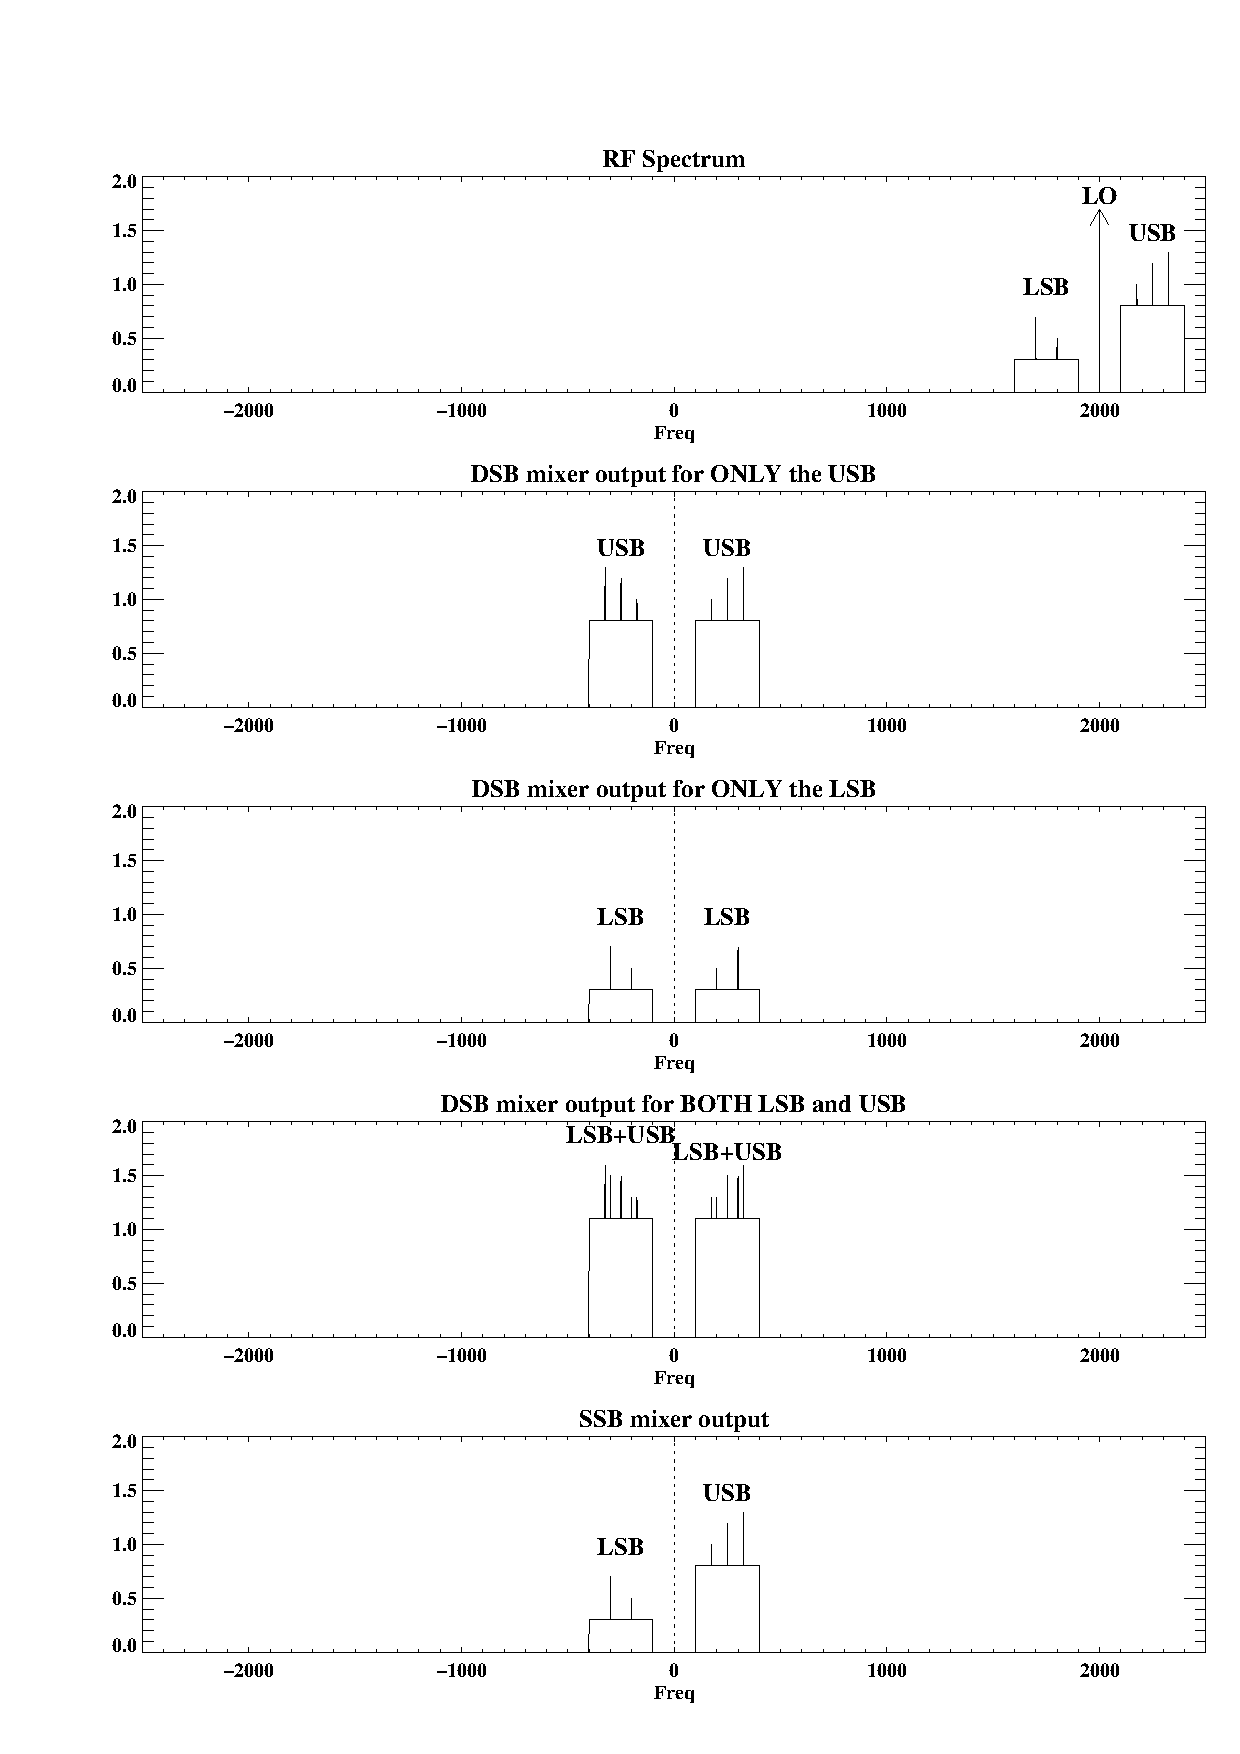
\includegraphics[width=6.5in]{sideband.png}
%\end{center}
%\hspace{-0.5in}
\caption{Upper (USB) and lower (LSB) sidebands in DSB and SSB mixers for a set of
test tones on top of broad level noise spectra. Panel 1 illustrates
  the RF
spectrum; panels 2 and 3 show the USB and LSB individually when
they undergo the DSB mixing process; panel 4 shows how they both add
together; panel 5 shows how the SSB mixer keeps them
separate. \label{sideband}}
\end{figure}
%
%Three things are important here:
%\begin{enumerate}
%
%\item The two sidebands---the two different input
%frequencies ($[\omega_{s-}= \wLO  - \Delta \omega]$ and $[\omega_{s+}=
%\wLO  + \Delta \omega]$)--- produce the same
%symmetric-around-zero pair of IF output frequencies $\pm |\Delta
%\omega|$. The DSB mixer
%cannot distinguish between the two input frequencies.
%
%\item Consider how $|\Delta \omega|$ depends on $\wLO $: for
%          the upper sideband, ${d |\Delta \omega| \over d\wLO } = -1$,
%          while for the lower $d {|\Delta \omega| \over d\wLO } =
%          +1$. We hope that the upper three panels of Figure
%          \ref{sideband} elucidate the situation.
%
%\item A value of $E_s$ for one sideband produces a certain mixer
%output power; the same value of $E_s$ for the other sideband
%produces the same power. With regard to power, the sidebands are {\it
%indistinguishable}.
%
%\end{enumerate}
%
%\noindent
Figure \ref{sideband} illustrates the result. The top panel shows the
original RF spectrum, which consists of signals above the LO (the upper
sideband; USB
signal) and below (the lower sideband; LSB). Suppose you use a filter to
eliminate the LSB, leaving only the USB. The second panel
shows the IF spectrum after DSB mixing: the USB appears at both negative
and positive frequencies and the spectrum is symmetric, meaning that the
negative frequencies give exactly the same result as the positive ones.

Now use a filter to eliminate the USB, leaving only the LSB;
the third panel shows the resulting IF spectrum.

Without any filters, then both the LSB and the USB
would appear in the IF spectrum, as in the fourth panel. 
With a DSB mixer, you can't distinguish between LSB and
USB. They are inextricably
mixed into a sum in the power spectrum.
However, the bottom panel shows that SSB 
mixing retains the sideband separation.

\section{Writing the Lab Report (Week 3)} \label{report}

\noindent
Please review the resources linked on AstroBaki and the guidelines
offered in class for generating your report. Remember that your write-up
is the basis for the majority of your grade in this class; make sure to
include high-quality plots and description, providing adequate background
and discussion such that one of your peers who has not taken this class would
be able to understand your findings and conclusions. Take the opportunity to
show off what you have learned so far!

Your report should directly address the goals listed in \S\ref{goals}, but
please ensure that you do so in a narrative that is directed toward the goal
of conveying high-level results.  It would be a mistake to make this report a
laundry-list of the things you did during the last couple of weeks. Not every
plot you made needs to be in this report, nor should every wrong turn be documented.
A scientific publication documents process, but only insofar as is necessary
to generate the results presented.

Finally, heed the warning that write-up takes longer than you think it will. Get
started early and allow yourself plenty of time.

%\subsection{Handouts}
%
%\begin{enumerate}
%\item What should your lab report look like? {\tt
%  labreport\_comments.pdf} {\it ``SUGGESTIONS FOR LAB REPORTS''}
%
%\item You must use \LaTeX for your lab report! {\tt sample.pdf} ``\LaTeX
%  Is Your Friend OR ENEMY?'' Answer to this question is a
%  resounding YES for `Friend'---if you have followed his handout. Use
%  \LaTeX for preparing your lab report!
%
%\item Now's the time for another look at efficient use of your text
%  editor, because if you learn the keystroke commands you'll be much
%  quicker and save lots of time further down the road.
%
%\item You'll need to show plots into your lab report. To do this you
%  make PDF files of your plots. %See {\tt bpidl.pdf} {\it ``BPPython---BASIC PLOTTING IN
%  %Python: PLOTS, MULTIPLE PLOTS, COLORS, MAKING POSTSCRIPT FILES''} Section 6.0.1.
%
%\end{enumerate}
\end{document}
